\documentclass[conference]{IEEEtran}

\usepackage[T1]{fontenc}
\usepackage[utf8]{inputenc}
\usepackage{amsmath}
\usepackage{booktabs}
\usepackage{graphicx}
\usepackage{microtype}
\usepackage{url}
\usepackage{xurl}
\usepackage[hidelinks]{hyperref}

\graphicspath{{./}{paper/}}

\title{DEEDY: A Thai-Centric Multi-Agent Framework and\\
Experimental Testbed for Public Sentiment Simulation}

\author{\IEEEauthorblockN{Sawit Koseeyaumporn}
\IEEEauthorblockA{Department of Computer Engineering\\
King Mongkut's University of Technology Thonburi, Bangkok, Thailand\\
\texttt{sawit.kosee@kmutt.ac.th}}}

\begin{document}
\maketitle

\begin{abstract}
This paper presents DEEDY (Digital Environment for Emergent Dynamics and
Yield), an application and experimental testbed for simulating Thai online
public discourse with large-language-model (LLM) agents. DEEDY turns event
descriptions, Thai news, forum discussions, and social-media traces into two
strictly separated products: a reality seed used to construct a simulated
world, and held-out observations used to test that world. Its data preparation
pipeline discovers topic-relevant sources, scrapes and records their
provenance, builds Thai-aware clean views, and produces structured summaries,
sentiment, stance, and sarcasm annotations. A MiroFish-based core then extracts
entities and relations, creates graph-grounded actors and environments, runs
OASIS social interactions, and emits auditable posts, actions, trajectories,
and reports. The proposed experiments evaluate whether the application
reproduces held-out Thai discourse at content, population, and diffusion
levels, rather than accepting linguistic plausibility as behavioral validity.
The evaluation combines sentiment and stance distribution distance, narrative
coverage, diversity, propagation error, network statistics, repeated runs,
Thai human ratings, and calibrated LLM-assisted judging. DEEDY is intended as
an exploratory social-listening and counterfactual-analysis instrument, not as
a substitute for Thai participants or a deterministic predictor of public
opinion.
\end{abstract}

\begin{IEEEkeywords}
LLM agents, agent-based modeling, social simulation, Thai NLP, public
sentiment, GraphRAG, MiroFish
\end{IEEEkeywords}

\section{Introduction}

Public opinion on social media emerges from interaction. A post is exposed by
a platform, interpreted through a user's prior beliefs and social identity,
answered or ignored, and then amplified through further recommendations. The
resulting narratives, sentiment shifts, polarization, and information cascades
cannot be reduced to independent text classifications. Agent-based modeling
(ABM) offers a bottom-up method for representing these local decisions and
observing the collective patterns that they produce~\cite{macal2010tutorial}.

LLM agents extend ABM by allowing an actor to condition open-ended actions on
a profile, memory, retrieved evidence, and conversational context. Generative
Agents demonstrated memory-driven believable behavior~\cite{park2023generative},
and Social Simulacra showed how generated users and conversations can populate
social-computing prototypes~\cite{park2022social}. Large-scale systems such as
$S^3$, OASIS, and GenSim subsequently modeled social networks, recommendation,
and diverse online actions~\cite{gao2023s3,yang2024oasis,tang2025gensim}.
MiroFish packages this capability as a document-to-simulation workflow:
reality-seed documents are converted into a knowledge graph, actors and an
environment are generated, OASIS executes the social simulation, and a report
agent interrogates the resulting world~\cite{mirofish2026}.

These capabilities are useful for Thai social listening, but two methodological
problems remain. First, Thai localization is more than translating an English
prompt. Thai has no obligatory whitespace between words, and online messages
contain informal spelling, repeated characters, emoji, hashtags, transliterated
English, regional language, sarcasm, indirect disagreement, and culturally
specific politeness. Thai NLP resources and models have improved
substantially~\cite{arreerard2022survey,phatthiyaphaibun2023pythainlp,
lowphansirikul2021wangchanberta,pipatanakul2024typhoon2}, but cultural capability
is still a separate evaluation target~\cite{kim2025thaicli}.

Second, a plausible post is not evidence that an agent behaves like the person
or population it represents. Demographically conditioned LLM samples can
approximate some human distributions~\cite{argyle2023out}, yet recent work finds
behavioral inconsistency across settings~\cite{mooney2025coherent}. Operational
validation against authentic comments also reveals that matching surface form
can be decoupled from matching content~\cite{schwager2026conditioned}. A social
simulator therefore requires held-out real observations, repeated runs, and
measurements at both individual and collective levels.

This paper introduces \textbf{DEEDY}, a Thai-centric application that joins a
data-preparation pipeline with the MiroFish core and an explicit experimental
validation layer. The application supports three practical uses: (i) auditing
how a Thai online debate may develop inside a controlled simulated environment,
(ii) comparing counterfactual message framing, actor composition, network, or
recommendation policies, and (iii) producing a traceable report that states
where simulated and observed discourse agree or diverge. It does not claim to
forecast Thai society as a whole.

Our contributions are threefold:
\begin{itemize}
    \item We develop an end-to-end Thai social-data pipeline that connects
    topic discovery, multi-source collection, provenance, Thai-aware text
    views, and structured weak annotation to graph-grounded simulation.
    \item We adapt the MiroFish/OASIS workflow to Thai public discourse through
    context-preserving actor construction, Thai linguistic attributes, and
    auditable simulation outputs suitable for an application rather than a
    one-off demonstration.
    \item We define a leakage-resistant experimental protocol that tests
    content, population, and dynamic correspondence against held-out Thai posts
    and comments, with ablations, repeated runs, human evaluation, and
    uncertainty reporting.
\end{itemize}

\section{Related Work}

\subsection{Generative Agents and Social Simulation}

Traditional ABMs encode actor states and behavioral rules explicitly. LLM
agents complement this approach by generating context-dependent language and
actions, but introduce sensitivity to prompts, decoding, memory, and the shared
base model. Generative Agents use observation, reflection, and planning to
produce coherent-seeming routines~\cite{park2023generative}. $S^3$ connects LLM
perception and action to emotion, attitude, and a social network
~\cite{gao2023s3}. OASIS adds dynamic user and post state, follow/comment/repost
actions, and configurable interest- and popularity-based recommendation at
large agent scales~\cite{yang2024oasis}. GenSim emphasizes reusable scenario
functions and execution robustness~\cite{tang2025gensim}. DEEDY uses these
systems as infrastructure, but focuses on Thai event construction and
empirical validation rather than maximum population size.

\subsection{Grounding and Operational Validity}

MiroFish extracts entities and relations from uploaded reality seeds, stores
individual and collective memory in a graph-retrieval layer, generates OASIS
profiles, runs social platforms, and uses a report agent to query simulation
state~\cite{mirofish2026}. This workflow accelerates scenario construction, but
the generated report is still evidence about the simulated world, not evidence
that the world is valid. DEEDY therefore treats every simulation trace as a
hypothesis to compare with unseen observations.

Algorithmic fidelity compares LLM-generated and human subgroup distributions
~\cite{argyle2023out}. Conditioned Comment Prediction instead compares a
generated response with the authentic response a user left to a stimulus,
providing a closer operational test for social-media simulation
~\cite{schwager2026conditioned}. Validation of generative ABMs further benefits
from staged replication before novel counterfactual tests
~\cite{cross2025validating}. These ideas motivate DEEDY's event-level holdout:
source material required to describe the event is available to agents, whereas
the reactions used for scoring are not.

\subsection{Thai Online Language and Public Sentiment}

Thai NLP remains comparatively resource-constrained, especially for informal
and downstream semantic tasks~\cite{arreerard2022survey}. PyThaiNLP provides
tokenization and other open Thai processing components
~\cite{phatthiyaphaibun2023pythainlp}; WangchanBERTa showed that Thai-specific
preprocessing and pretraining over news and social data matter
~\cite{lowphansirikul2021wangchanberta}; and Typhoon 2 extends Thai-optimized
models to instruction-following generation~\cite{pipatanakul2024typhoon2}.
ThaiCLI separately evaluates cultural and linguistic knowledge, highlighting
that general benchmark strength does not guarantee Thai cultural competence
~\cite{kim2025thaicli}.

Online affect is also contextual. Sarcasm can invert literal polarity, and
conversation history and user style improve its detection
~\cite{hazarika2018cascade}. This is important in Thai discussions, where
particles, quotation, exaggerated praise, wordplay, and shared cultural
references may signal stance indirectly. Accordingly, DEEDY keeps thread
context and raw text for evaluation and does not treat sentiment, stance, and
sarcasm as interchangeable labels.

\section{DEEDY Framework}

\begin{figure*}[t]
    \centering
    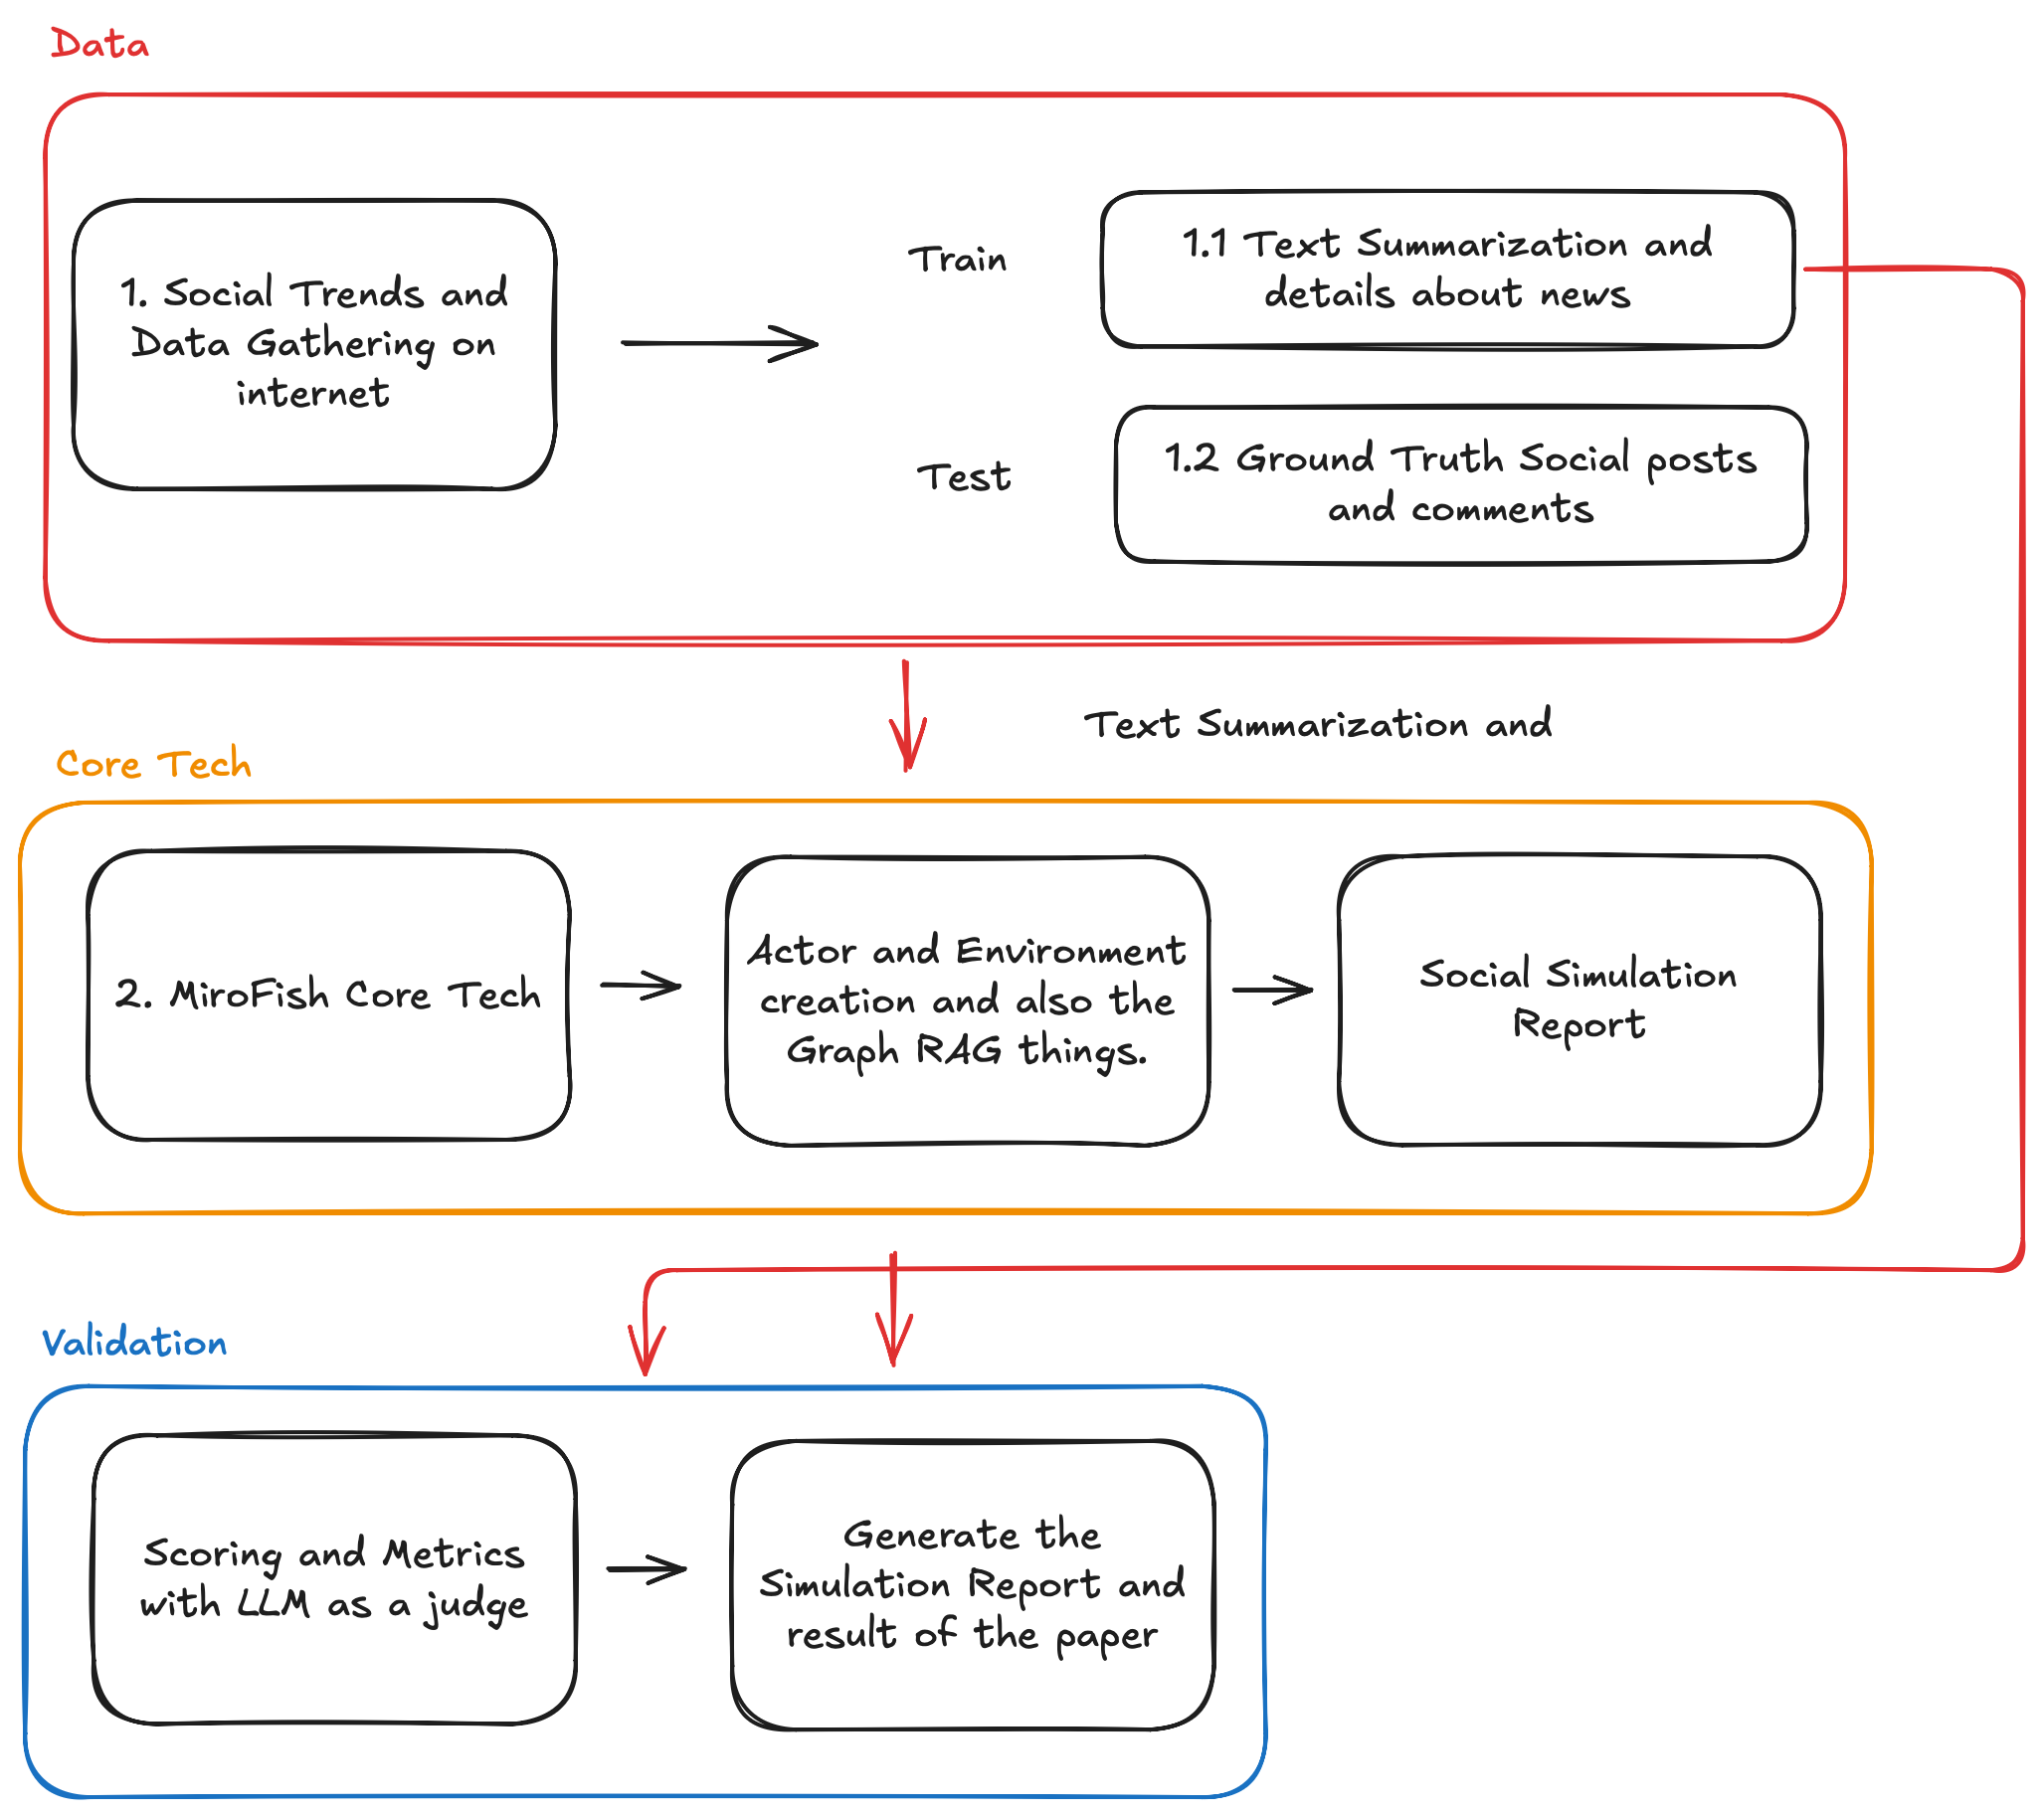
\includegraphics[width=0.78\textwidth]{system_arch.png}
    \caption{DEEDY application architecture. Topic-relevant Thai web data are
    separated into a scenario-construction stream and a held-out validation
    stream. The MiroFish core builds a graph-grounded environment and actors,
    runs social simulation, and exposes outputs for multi-level evaluation.}
    \label{fig:deedy-architecture}
\end{figure*}

\subsection{System Architecture Overview}

Figure~\ref{fig:deedy-architecture} organizes DEEDY into three layers. The
\emph{data layer} discovers, collects, cleans, partitions, and annotates Thai
event material. The \emph{core layer} supplies the scenario summary to
MiroFish, which constructs a GraphRAG-backed world, creates heterogeneous
actors, executes social interactions, and generates a simulation report. The
\emph{validation layer} compares outputs with social posts and comments never
shown to the agents. Every derived artifact records a topic identifier, source
type, provenance pointer, processing version, and experimental split so that a
score can be traced back to its evidence.

\subsection{Data Preparation Pipeline}

\subsubsection{Topic and Source Discovery}

Topics are defined in \texttt{data/topic.json} as a Thai debate statement and
a list of search expressions. The current corpus contains 29 topics spanning
everyday culture, public services, work, mobility, tourism, education, and
policy. Examples include authentic ingredients in \emph{pad kaphrao}, dowry,
motorcycles on footpaths, school uniforms, fare affordability, free overtime,
and cannabis policy. This topic-first design deliberately samples contested
issues with at least two recognizable stances rather than claiming a random
sample of all Thai conversation.

The discovery stage provides two implementations. The legacy queue uses Google
News RSS together with Pantip search and TikTok search URLs. The revised
\texttt{discover\_v2.py} replaces the news dependency with DuckDuckGo news/web
search localized to \texttt{th-th} and a Bing News RSS fallback, while retaining
Pantip's native search endpoint with an HTML fallback. URLs are de-duplicated
within topic and stored as JSON Lines. A source URL is a candidate, not yet a
valid observation; relevance, accessibility, duplicates across topics, and
publication time are checked downstream.

\subsubsection{Collection and Provenance}

\texttt{drama\_crawler.py} routes each candidate to a source adapter. News and
general pages are redirect-resolved, downloaded, parsed with BeautifulSoup,
and converted to Markdown. If a page is blocked, the implementation attempts a
Wayback Machine snapshot. The Pantip adapter extracts the topic title, main
post, and available comment blocks. TikTok is currently only a dynamic-page
hook: the requests-based crawler records a placeholder and does not retrieve
comments. TikTok records are therefore excluded from experiments until a
rendered, policy-compliant adapter and stable provenance fields are implemented.

Each observation should retain the original URL, retrieval time, source type,
document title, raw text, and, where available, publication time, anonymized
author key, reply-parent key, and engagement counts. The final four fields are
required for propagation and network experiments. They are not present in the
current JSONL schema, so the first content experiment can proceed now, whereas
dynamic validation remains contingent on the trace-enriched crawler.

\begin{table}[t]
\caption{Data-pipeline snapshot inspected on 1 August 2026. Counts describe
the current working corpus and are not final experimental sample sizes.}
\label{tab:data-snapshot}
\centering
\footnotesize
\begin{tabular}{@{}lr@{}}
\toprule
Artifact & Current count \\
\midrule
Defined Thai debate topics & 29 \\
Discovered references & 709 \\
\quad Google News / Web / Pantip / TikTok & 411 / 27 / 242 / 29 \\
Topics in the scraped snapshot & 22 \\
Scraped items / non-empty items & 433 / 382 \\
Clean-view characters & 2,522,439 \\
\bottomrule
\end{tabular}
\end{table}

\subsubsection{Thai-Aware Text Views}

The implemented \texttt{text\_cleansing.py} retains Thai Unicode characters,
Latin letters, digits, ASCII/Markdown punctuation, and whitespace, while
removing emoji, other scripts, control characters, and encoding artifacts. It
also recovers records from either line-delimited JSON or concatenated JSON
streams. This produces a stable clean view for ingestion, but is intentionally
\emph{not} treated as a lossless representation. Emoji, script mixing,
orthographic repetition, and punctuation are possible affect or stance cues.

DEEDY consequently uses two synchronized views in the experimental design:
(i) an immutable raw view for annotation and held-out evaluation, and (ii) a
normalized ingestion view for graph construction. Normalization standardizes
encoding and whitespace but preserves hashtags, emoji as named features,
Thai--English code-mixing, negation, particles, and repeated-character counts.
Thai tokenization is performed only when a metric requires tokens; character-
and embedding-level metrics are reported in parallel to reduce dependence on a
single segmentation system.

\subsubsection{Evidence Split and Structured Weak Annotation}

For each topic $e$, the collected evidence is partitioned before any model
summary is generated:
\begin{equation}
    D_e = S_e \;\dot\cup\; G_e,
\end{equation}
where $S_e$ is the scenario-construction set and $G_e$ is held-out ground
truth. $S_e$ contains event facts available before the validation window,
primarily news and official context. $G_e$ contains subsequent posts, comments,
and interactions. Near duplicates are clustered before splitting, and a source
or quoted passage cannot occur in both sets. Event and post timestamps enforce
a temporal cut when available.

\texttt{llm\_labels\_fusion.py} currently sends up to ten cleaned sources per
topic to OpenRouter Fusion and requests a factual summary, public-opinion
direction, polarization axis, and micro labels for sentiment, stance, and Thai
sarcasm. Sentiment ratios are then computed deterministically from micro-label
counts. These outputs are \emph{weak pre-annotations}, not ground truth. Before
the main experiment the script will operate separately on $S_e$ and $G_e$;
only the summary derived from $S_e$ enters MiroFish, while labels for $G_e$ are
reviewed by Thai annotators and used only for scoring. This change prevents the
current all-sources fusion path from leaking validation reactions into actor
memory.

\subsection{MiroFish Core Engine}

\subsubsection{Reality Seed and GraphRAG}

The scenario packet contains the event summary, dated factual claims, named
entities, organizations, locations, and source-level provenance from $S_e$.
MiroFish extracts an ontology and entity relations, then injects individual and
collective memories into its graph retrieval layer~\cite{mirofish2026}. A
retrieved memory attached to an agent action includes its supporting node or
source identifier. Unsupported details generated during graph construction are
marked as model assumptions and are not silently promoted to facts.

\subsubsection{Actor and Environment Construction}

Actors represent roles observed or justified by $S_e$, such as affected
citizens, service providers, institutions, advocates, bystanders, media, and
domain experts. A profile separates evidence-backed attributes from sampled
attributes. The Thai adaptation adds language register, Thai--English mixing
rate, region/dialect only when supported, politeness strategy, typical message
length, activity rate, stance prior, interests, and uncertainty. Demographic
attributes are not inferred from a single message. Population weights and
network links are sampled from documented priors and varied during sensitivity
analysis rather than presented as known facts.

The environment specifies platforms, action space, time step, feed capacity,
and recommendation mechanism. OASIS supplies posting, replying, reposting,
following, and browsing behavior with dynamic social and content state
~\cite{yang2024oasis}. DEEDY additionally records each exposure before an
action. This makes it possible to distinguish ``the agent never saw the
message'' from ``the agent saw and rejected the message,'' a necessary
distinction for interpreting diffusion failure.

\subsubsection{Thai Context in Perception and Action}

At each round, an actor retrieves relevant graph memory, observes a bounded
feed, updates a private state, and chooses an action or abstention. Prompts
require natural Thai consistent with the actor's register without demanding
caricatured dialect. They preserve uncertainty, allow silence, and prohibit
fabricated quotations or demographic claims. Conversation context is included
for reply generation because Thai stance and sarcasm may depend on an earlier
turn~\cite{hazarika2018cascade}. The language model is configurable: a
Thai-optimized model such as Typhoon 2 and a strong multilingual model are
compared under identical action rules rather than assuming either is superior.

\subsubsection{Simulation Outputs and Application Layer}

The core returns a machine-readable event log and a human-readable report. The
log contains agent state version, exposure set, retrieved evidence, selected
action, generated content, parent action, timestamp, and token/model settings.
The report summarizes dominant and minority narratives, sentiment and stance
trajectories, influential nodes, propagation paths, disagreement, and
unsupported claims. It also exposes uncertainty across runs.

The application allows an analyst to select an event, inspect the scenario
packet and graph, configure actor count and feed policy, run a baseline or
counterfactual, compare it with held-out observations, and drill down from an
aggregate chart to the posts and evidence that produced it. Counterfactual
reports compare conditions inside the model; they are not presented as causal
effects in the real Thai population.

\section{Experimental Design}

\subsection{Research Questions}

The evaluation is organized around four questions:
\begin{itemize}
    \item \textbf{RQ1 (Content):} Does DEEDY reproduce the sentiment, stance,
    narrative, and linguistic characteristics of held-out Thai reactions?
    \item \textbf{RQ2 (Population):} Does graph grounding and Thai adaptation
    improve aggregate correspondence without collapsing response diversity?
    \item \textbf{RQ3 (Dynamics):} Does the simulated interaction process match
    observed cascade size, shape, timing, and network structure?
    \item \textbf{RQ4 (Application):} Are reports traceable, stable across
    repeated runs, and useful to Thai analysts without overstating certainty?
\end{itemize}

\subsection{Dataset and Splitting Protocol}

The initial study will select topics with at least five usable scenario sources
and a minimum held-out reaction count fixed before inspection of outputs. The
unit of generalization is an \emph{event}, not a post: all tuning and prompt
selection use development events, and final scores are reported on untouched
test events. Within an event, a timestamped source split separates $S_e$ from
$G_e$. If timestamps are unavailable, the event may be used for content-pilot
analysis but not for a prospective or diffusion claim.

Weak labels are independently reviewed by at least three native Thai
annotators using a codebook for three-way sentiment, event-specific stance,
sarcasm, and narrative membership. Annotators see necessary conversational
context but not whether a post is real or simulated during quality comparison.
Majority/adjudicated labels form the reference set, and Krippendorff's
$\alpha$ is reported for each task. User identifiers are hashed and quoted
examples are paraphrased unless publication is ethically justified.

\begin{table*}[t]
\caption{Planned experiments. Each condition is run with the same event split,
agent budget, round budget, and ten random seeds unless that factor is varied.}
\label{tab:experiments}
\centering
\footnotesize
\begin{tabular}{@{}p{0.16\textwidth}p{0.31\textwidth}p{0.43\textwidth}@{}}
\toprule
Experiment & Conditions & Primary purpose \\
\midrule
Exp. 1: Grounding & DEEDY seed-only; ungrounded LLM agents; deliberately leaky
all-source upper bound & Test whether held-out correspondence comes from the
scenario pipeline rather than parametric knowledge or target leakage. \\
Exp. 2: Thai adaptation & Full Thai adaptation; translated/unadapted MiroFish;
normalization without context features & Measure sentiment/stance distance,
narrative coverage, Thai quality, sarcasm, code-mixing, and diversity. \\
Exp. 3: Core model & Thai-optimized LLM; matched multilingual LLM; simple
non-generative ABM baseline & Separate the contribution of the language model
from the graph, population, and platform mechanisms. \\
Exp. 4: Social mechanism & Chronological, popularity, and interest feeds;
observed versus random network; multiple population sizes & Test cascade,
polarization, herding, and sensitivity to platform assumptions. \\
Exp. 5: Application & Baseline event versus one pre-registered message-framing
counterfactual; report with versus without uncertainty/evidence links & Assess
traceability, analyst usefulness, and whether presentation changes trust. \\
\bottomrule
\end{tabular}
\end{table*}

\subsection{Metrics}

\subsubsection{Content and Population Correspondence}

Let $P_G^y$ and $P_S^y$ be observed and simulated distributions for label
$y\in\{\text{sentiment},\text{stance},\text{narrative}\}$. Distributional
correspondence is measured with Jensen--Shannon distance:
\begin{equation}
 d_{\mathrm{JS}}(P_G^y,P_S^y)=
 \sqrt{\tfrac{1}{2}D_{\mathrm{KL}}(P_G^y\Vert M)+
 \tfrac{1}{2}D_{\mathrm{KL}}(P_S^y\Vert M)},
\end{equation}
where $M=(P_G^y+P_S^y)/2$. Lower is better and the square-root form is bounded.
Macro-F1 is also reported when simulated posts are matched to a conditioned
stimulus or stance target.

Narrative correspondence is measured in two ways. First, Thai annotators map
posts to an event-specific narrative codebook and we compare coverage and
prevalence. Second, multilingual BERTScore measures semantic similarity between
generated and observed response sets~\cite{zhang2020bertscore}. Embedding-based
scores are treated as complementary because semantic proximity need not imply
the same stance. Diversity is reported using Distinct-1/2, Self-BLEU, unique
narrative count, lexical entropy, length distribution, and pairwise embedding
distance. High correspondence accompanied by diversity collapse is considered
a failure.

Polarization is measured from the stance distribution and interaction graph.
We report normalized stance entropy, between-group versus within-group
interaction, and modularity after fixing the community-detection procedure.
Population statistics are computed per run and then aggregated across events,
so events with many scraped posts do not automatically dominate the result.

\subsubsection{Temporal and Network Correspondence}

For trace-enriched topics, cumulative activity curves are aligned to the event
start. We report normalized root-mean-square error (NRMSE) and dynamic time
warping distance, together with cascade scale, maximum depth, maximum breadth,
structural virality, time to 50\% of final activity, and peak-time error. OASIS
uses scale, depth, breadth, and propagation-curve error in its own validation
~\cite{yang2024oasis}; DEEDY adds exposure-conditioned action rates and Thai
content labels.

Observed and simulated interaction graphs are compared by degree and cascade-
size distributions using the two-sample Kolmogorov--Smirnov statistic, plus
clustering coefficient, reciprocity, assortativity, modularity, and the share
of cross-stance replies. These metrics are omitted, rather than imputed, when
the source platform does not expose the required trace.

\subsubsection{Thai Quality and Report Evaluation}

Native Thai raters score blinded real and simulated posts on a five-point scale
for naturalness, contextual coherence, stance consistency, pragmatic and
cultural appropriateness, and persona consistency. Sarcasm precision, recall,
and F1 are evaluated separately. Report claims are scored for evidence
traceability: the proportion of factual claims linked to scenario evidence or
simulation events, unsupported-claim rate, contradiction rate, and coverage of
minority narratives.

An LLM judge may assist high-volume screening, but cannot be the sole quality
measure. Pair order is swapped, output identity is hidden, the judge must cite
the supplied evidence before scoring, and its agreement with Thai raters is
reported. These controls address known position bias in LLM-as-a-judge
evaluation~\cite{shi2024judging}.

\subsection{Execution and Statistical Analysis}

All stochastic conditions use ten seeds initially; a power analysis on pilot
variance determines the final number. Model name and revision, prompts,
temperature, top-$p$, agent count, network seed, recommendation parameters,
round count, stopping rule, and token cost are frozen before the test set is
opened. We report medians and 95\% bootstrap confidence intervals across
events. Paired conditions use an event-level permutation test or Wilcoxon
signed-rank test with Holm correction. Effect sizes accompany $p$-values.

The main comparison is the full DEEDY pipeline versus translated/unadapted
MiroFish. Component ablations remove graph retrieval, Thai context features,
thread context, or observed population weights one at a time. The deliberately
leaky condition in Table~\ref{tab:experiments} is never a valid system result;
it is a diagnostic ceiling showing how much apparent performance can be gained
by exposing held-out reactions.

\subsection{Acceptance Criteria for the Application}

Before results are observed, the study will set minimum criteria: (i) full
pipeline completion and provenance for every scored run; (ii) statistically
lower sentiment/stance Jensen--Shannon distance than the unadapted baseline;
(iii) no significant diversity collapse relative to held-out posts; (iv) Thai
quality above the midpoint with acceptable annotator agreement; (v) report
unsupported-claim rate below a pre-registered threshold; and (vi), for
trace-enriched events, improvement on at least two cascade metrics without
material degradation on the others. Failure remains a reportable result and
defines the application's operating boundary.

\section{Limitations and Ethical Considerations}

The present corpus is a convenience sample driven by search terms and public
web accessibility. It over-represents searchable news and Pantip, does not yet
contain usable TikTok comments, and cannot represent the Thai population.
Source deletion, search ranking, crawler failure, coordinated activity, bots,
and platform-specific moderation may bias observed discourse. The current
cleaner also removes emoji and other scripts; experiments must use the paired
raw/context-preserving view before making linguistic claims.

Personas can reproduce stereotypes even when generated from real traces.
DEEDY therefore avoids inferring sensitive attributes from isolated posts,
reports subgroup results only where data and ethics permit, and presents
regional or dialect attributes as uncertain rather than essential. Public
availability does not remove privacy risk: identifiers must be hashed, raw
text access restricted, quotations minimized, and collection reviewed against
platform terms and institutional research-ethics requirements.

Finally, LLM agents share training data, architecture, and prompt conventions;
agreement between them may reflect a common model prior rather than social
consensus. Counterfactual findings are conditional on the scenario, actor
sampling, network, recommender, and model version. DEEDY is therefore an
instrument for exploratory comparison and hypothesis generation, not a
replacement for surveys, field studies, or participatory research with Thai
communities.

\section{Conclusion and Future Work}

\emph{Placeholder---to be completed after the data pipeline, MiroFish core,
and experiments are finalized. The final conclusion will summarize measured
findings, supported application claims, failure cases, and next steps without
introducing results that are not reported in the paper.}

\bibliographystyle{IEEEtran}
\bibliography{deedy_references}

\end{document}
